\subsection{Source ceramic gas-face partition and remaining closure}
The nominal and taller assemblies have identical source ceramic face areas and 0.600 and 0.700 mm substrate gaps, respectively. Direct metal contact on each ceramic face is partitioned from bare regions, and bare regions are divided into the projection facing the adjacent plate and the remaining area. This is a face-area accounting result, not a three-dimensional gas path or a gas transfer coefficient. For the three lower faces in each interstage gap, direct-contact-free facing areas are 11.218, 8.072 and 3.215 mm$^2$; on the opposing upper faces they are 11.380, 8.500 and 3.600 mm$^2$. Patterned metal covers different parts of each face. Gas can also contact those metal surfaces, so bare ceramic areas alone cannot represent total transfer.

The source cap, roof and window are present as ideal solids, and an earlier nominal derived geometry contains a connected gas volume. The taller assembly has not yet received an independently qualified connected-gas and complete gas-facing metal-port mapping. Its seal and gas transport parameters are not measured. Treating the projected ceramic regions as independent gas paths would therefore omit metal and could still double-count connected gas transport. No new paired temperature solve was made, and the preceding conditional comparisons retain their limitations.

\begin{figure}[htbp]\centering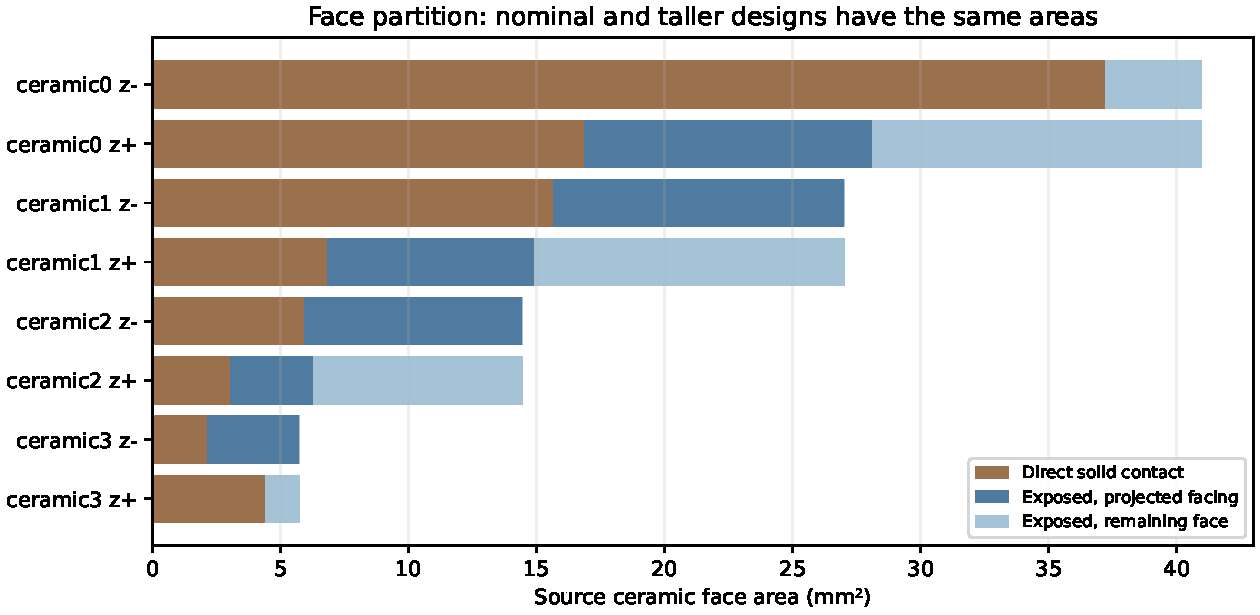
\includegraphics[width=.94\linewidth]{figures/v322_gas_face_partition.pdf}\caption{Disjoint rectangular source-ceramic face areas for the two assemblies. ``Facing'' indicates only the projection of the neighbouring ceramic onto the bare face, not free access through the gap. The source side faces and gas-facing metallization are not shown.}\end{figure}
